\chapter{Europium}\label{ch:europium}

Europium is a peculiar metal. As a lanthanide metal, it has a complex
electronic structure consisting of an incomplete \textsl{4f} electron shell
that is highly reactive \cite{Cooley:1946tv,Rard:1985tb}. These two properties create a
tricky spectroscopic problem: europium has very low absorption cross sections
in the visible due to its electronic structure, and europium's reactivity means
that it is difficult to acquire lone europium to detect. This means that to
analyse europium in a solution it must be present at relatively high
concentration in a medium that europium does not react with.

\marginpar{Lower concentrations of europium can be measured in the UV.}

Using \ac{BBCEAS} it is possible to detect europium in a liquid sample at lower
concentrations than what is published in the literature.  The broad spectral
and simultaneous acquisition nature of \ac{BBCEAS} allows several spectral
features in the visible to be measured simultaneously.

While europium is challenging to characterise, it has a immensely valuable
property: europium's photoluminescent quantum yield is nearly one
\cite{Scotognella:2009jo,Moudam:2009in, Bunzli:2005ic}, and the fluorescence
emission can be spectrally very narrow \cite{Werts:2002fs}. The quantum yield
is an important parameter in engineering uses for europium, yet this property
has not been explored well in the past due to the difficulty of extracting
information from fluorescence measurements \cite{Werts:2002fs}. By measuring
the absorption characteristics of europium using \ac{BBCEAS}, it is possible to
obtain a greater understanding of the fluorescence pathways and how to alter
them.

Europium also readily forms coordination complexes as both monodentate and
polydentate ligands
\cite{Kirby:1983cl,Sveshnikova:2000cr,Werts:2002fs,Bunzli:2005ic,Scotognella:2009jo,Moudam:2009in}. The fluorescence of europium, combined with a coordination complex, can be used
to create sensitive labels
\cite{Harma:2010dm,Pihlasalo:2010el,InstituteofBiomedicine:2011vt,Pihlasalo:2011ju,Pihlasalo:2012cq,Pihlasalo:2012en},
to create OLEDs with high spectral purity\cite{Moudam:2009in}, and as
luminescent solar concentrators\cite{Moudam:2009in,Wilson:2010hs}.

This chapter will explore the current understanding of europium's electronic
transitions and how to derive additional information such as quantum yields and
radiative lifetimes about europium complexes using \ac{BBCEAS}. Near the end is
a discussion about how it is possible to combine \ac{BBCEAS} with europium
complexes to create a highly sensitive protein detection technique that can not
only detect trace concentrations of proteins but also indicate which proteins
are in a solution.



\section{Theory of Lanthanide electronic transitions}\label{sec:theory_eu}

Lanthanide ions contain an open \textsl{4f} electronic orbital which leads to
many strange phenomena that are difficult to describe with standard quantum
mechanical models\cite{Wybourne:1968ez}. In the 1960s, researchers Judd and
Ofelt introduced simple assumptions to make the calculation of the electronic
wave functions simpler \cite{Judd:1962uq,Ofelt:1962kd}.  Their simplifications
were immensely successful in theoretically predicting the energy levels of
different electron configurations.

However, there exist electronic transitions that are still difficult to
understand because they are classically \emph{forbidden}. Some transitions are
forbidden due to a transition between two ground total angular momentum states
(noted as $ J=0 \leftrightarrow J'=0 $), while many others are forbidden due to
a change in the total spin $\Delta S \neq 0$. As such, these transitions must
occur due to higher order effects, such as electron configuration interaction
for the $^7F_0 \leftrightarrow ^5D_0$ transition \cite{Jankowski:1981es}, These
transitions have much weaker absorption cross sections than classically allowed
transitions.



\subsection{Predicting Energy Levels in Europium}\label{subsec:predict_eu}

\begin{figure}
\begin{center}
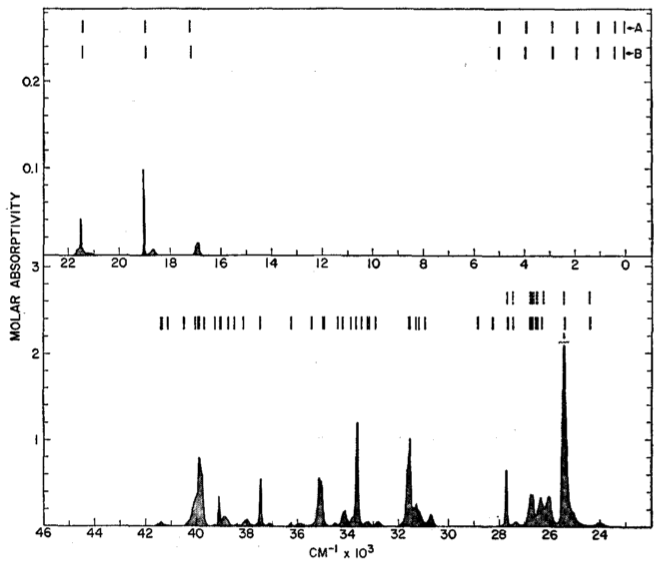
\includegraphics[width=\textwidth]{figures/eu_spec.png}
\end{center}
\caption{The expected absorption spectrum of aqueous europium from \cite{Carnall:1968ch}. The weaker, forbidden transitions are mostly seen in the visible, there they have an order of magnitude lower molar extinction.}
\label{fig:eu_spec_theory}
\end{figure}

It is possible, using extensions to Judd-Ofelt calculations, to derive the
energy levels of the \textsl{4f} energy shell and the transitions from the
ground state of europium in different mediums
\cite{Carnall:1968ch,Carnall:1989fc,Richardson:1989vf,vanPieterson:2002hd}.

\begin{align}
  H = H_{\text{free ion}} + H_{CF} \label{eq:lan_ham}
\end{align}

%\begin{align*}
%H =\ & H_0 + \sum_{k=2,4,6} F^kf_k \\
 %& + \zeta(4f)A_{so} + \alpha L(L+1) + \beta G(G_2) + \gamma G(R_7)\\
 %& + \sum_{i=2,3,4,6,7,8}t_iT^i + \sum_{h=0,2,4}m_hM^h + \sum_{f=2,4,6}p_fP^f
%\end{align*}

This equation represents the free ion Hamiltonian of a lanthanide ion.
$H_{\text{free ion}}$ is the non-interacting electrons contribution (known as
the barycenter) \cite{Peijzel:2005jh}. Accurate quantum mechanical models of
the free ion term are available in the literature and can be easily solved
numerically on a computer \cite{Carnall:1989fc,Morrison:1988tw}.

One can then add perturbation terms to alter the Hamiltonian for use in
different solutions. For example, if one has a solid crystal lattice, it is
common to add

\begin{align*}
  H_{CF} = \sum_{k,q} B_q^k C_q^{(k)}
\end{align*}

which represents the radial $B$ and many-electron spherical tensor $C$ crystal
field interaction with the electron wave functions \cite{Peijzel:2005jh}.  Some
forbidden excited states of europium can also be understood through the
Wybourne-Downer mechanism, which accounts for spin-orbit interaction among
excited states and explicitly allows for $\Delta S = 1$ transitions to occur
\cite{Wybourne:1968ez,Downer:1988kz}.  Finally, Judd-Ofelt theory can be used
to estimate the transition intensities and branching ratios of absorption and
emission spectra, and therefore the natural radiative lifetimes
\cite{Werts:2002fs}.



\subsection{Measuring Radiative lifetimes of Europium Complexes using Fluorescence Emission}\label{subsec:rad_life}

The radiative lifetime of an electronic transition of an absorber can be
determined by its emission profile \cite{Werts:2002fs}. This is done through
the following formula.

\begin{align}
  \frac{1}{\tau_R} = \sum_JA_{J'J}\label{eq:nat_life_emiss}
\end{align}

In this formula, $A$ is the spontaneous emission probability of a particular
$J' \leftrightarrow J$ transition\marginpar{$A$ is also known as the Einstein
$A$ coefficient} (which is related to the area under the curve for that
emission peak), and $\tau_R$ is the ``natural'' radiative lifetime, which is
the lifetime of an electron in an excited state without interference from
systematic effects such as thermal quenching. Additionally, one can define the
\emph{branching ratio} $\beta$ as the probability for an excited electron to
decay via a certain pathway $J_p$.

\begin{align}
  \beta_{J'J_P} = \dfrac{A_{J'J_p}}{\tau_R} = A_{J'J_p}\sum_J A_{J'J} \label{eq:branch_ratio}
\end{align}

For some absorbers, it can be difficult to measure all transitions
simultaneously, as some may be forbidden and hence extremely weak in comparison
to the allowed transitions. However, europium has a unique property that allows
its radiative lifetime to be determined from a single peak: europium contains a
single allowed magnetic dipole moment transition $^5D_0 \leftrightarrow ^7F_1$.
Magnetic dipole transitions are not affected by the solvent or complex than an
absorber is in, and hence this transition is constant \cite{Werts:2002fs}.
Using this peak, it is possible to measure the radiative lifetime using the
following equation

\begin{align}
  \dfrac{1}{\tau_R} = A_{MD,0}n^3\left(\frac{I}{I_{MD}}\right) \label{eq:nat_life_eu}
\end{align}

where $n$ is the refractive index of the solution, and the fraction
$\frac{I}{I_{MD}}$ is the ratio of the total area under the emission curve to
the area under just the $^5D_0 \leftrightarrow ^7F_1$ transition.

It is also possible, in cases where the absorption spectrum of a particular
luminescence transition is known, to calculate the radiative lifetime of the
transition \cite{Lewis:1945tp},

\begin{align}
  \frac{1}{\tau_R} = 2303 \dfrac{8\pi c n ^2 \nu^2}{N_A}\dfrac{g_l}{g_u}\int\epsilon(\nu)\,d\nu \label{eq:nat_life_abs}
\end{align}

where $\nu$ is the frequency of the transition, $\tfrac{g_l}{g_u}$ is the
fraction of electrons in the excited and ground state, and $\epsilon$ is the
molar extinction coefficient (in \iM\icm) of the transition.



\section{Experimental Liquid Eu(III) Results in the Literature}\label{sec:previous_eu_results}

Previous experiments have been able to detect small quantities of liquid
europium using absorption spectroscopy in the ultraviolet \cite{Yun:2001wc}.
However, the most interesting transitions for europium occur in the visible due
to the high efficiencies of the fluorescence decay pathway in europium. Under
these conditions, it is difficult to acquire an accurate absorption spectrum
for analysis of concentration or natural radiative lifetimes. To date, it
appears that within the visible the lowest concentration ever measured is
200\,mM of aqueous europium. This has been measured using complex
spectrophotometers and through \ac{PAS} \cite{Sawada:1979vca}.

These experimental results reveal a few interesting factors about europium's
electronic transitions (see Figure~\ref{fig:eu_spec_theory}. First, the
forbidden transitions are not much weaker than the allowed $^7F_0
\leftrightarrow ^5D_2$ transition near 464nm, which occurs when nonlinear
effects to the electronic wave functions play a dominant role
\cite{Walsh:2005te}. A second peculiarity was noted in the forbidden $^7F_0
\leftrightarrow ^5D_0$ transition, which found this absorption peak was
incredibly small in comparison to other transitions in the aqueous europium
spectrum \cite{Sawada:1979vca}. The authors who noted this peculiarity suggests
that the thinness is due to hypersensitivity of the transition to the
environment that the europium is in, leading to a squeezing effect of the
spectral line that overpowers the broadening effects.

It is important, especially for the applications discussed in
section~\ref{subsec:eu_beads}, to be able to detect aqueous europium at much
smaller concentrations than 200\,mM in the visible. As the proceeding
discussion shows, \ac{BBCEAS} is uniquely apt at being able to determine minute
quantities of aqueous europium in a way that provides qualitative data about
the fluorescence transitions that is most possible through other methods. As
such, the experimental setup designed in chapter~\ref{ch:bbceas} was used to
determine just how low of a limit of detection could be obtained with
\ac{BBCEAS}.



\section{Measurements using BBCEAS}\label{sec:eu_measurements}

\begin{figure}
\begin{center}
\includegraphics[width=\textwidth]{figures/eu_plot}
\end{center}
\caption{Europium absorption spectrum taken at different concentrations.}
\label{fig:eu_conc}
\end{figure}

\begin{figure}
\begin{center}
\includegraphics[width=\textwidth]{figures/eu_power_combined}
\end{center}
\caption{Europium absorption spectrum taken at different powers.}
\label{fig:eu_power}
\end{figure}

With experimental and theoretical results indicating what should be seen in an
absorption spectrum, the \ac{BBCEAS} technique was applied to measure small
concentrations of liquid europium in the visible, at concentrations lower than
the 200\,mM seen in the literature \cite{Sawada:1979vca}. This was accomplished
using the same technique used to perform the rhodamine 6G calibrations in chapter \ref{ch:cal}.

As one can see from figure~\ref{fig:eu_conc}, the major electronic transitions
were easily observed. However, as one can see from the figure, it is difficult
to determine why the measured spectrum has a higher baseline, and why the
relative intensities between the transitions do not match those in the
literature. Since the altering of the intensity of the different transitions
can occur when a substance is optically saturated, the experiment was repeated
at lower powers.

Figure~\ref{fig:eu_power} debunks the idea of optical saturation because the
signal appears nearly constant at many different input powers to the cavity,
even though the highest power in the set of the experiments is the same as the
original. This peculiar result is likely due to laser fluctuations in the
original liquid europium measurements (the laser fluctuation is a function of
time \emph{and} wavelength: see section~\ref{subsec:laser_fluc}).

Measurements were also performed on a variety of concentrations. This resulted
in a minimal detection limit of approximately 5\,mM in the visible, a 40 fold
improvement in the limit of detection against what is commonly seen in the
literature. This sensitivity is based on equation \eqref{eq:ceas_err_geo}.

These results indicate that \ac{BBCEAS} can be used to detect liquid Eu(III) at
a lower concentration than what was possible before. With modifications to the
\ac{BBCEAS} setup (discussed in section~\ref{sec:bbceas_enhance}) it will be
possible to lower the detectable concentration to the micromolar range.



\section{Further Investigations of Europium}\label{sec:eu_future}

In this chapter it has been shown that preliminary \ac{BBCEAS} testing of
Eu(III) in aqueous solution can be detected in much smaller quantities than
previously reported in the literature.  This detection limit, combined with
coordination complexes, can be used to better understand europium complexes and
to illuminate how to use such complexes effectively.



\subsection{Europium Complexes}\label{subsec:eu_complex}

It is quite tricky to measure the absorption spectrum of europium and detect
any fluorescence due to the extremely low absorption cross sections of the
europium ion. Coordination complexes alleviate this problem by acting as
``catcher's mitts'', which dramatically increases the probability of a photon
being absorbed
\cite{Kirby:1983cl,Sveshnikova:2000cr,Werts:2002fs,Bunzli:2005ic,Moudam:2009in,Wilson:2010hs,Harma:2010dm,InstituteofBiomedicine:2011vt,Pihlasalo:2012cq}.
Combined with the high fluorescence quantum efficiency of the europium
complexes, these coordination systems increase the usability of europium by
allowing even moderate intensity light sources to induce fluorescence of high
spectral purity.

However, to calculate the theoretical parameters for such a system, it is
necessary to measure the time required for an excited europium complex to decay
down to the ground state. As shown from equations \eqref{eq:nat_life_emiss},
\eqref{eq:nat_life_abs} and \eqref{eq:branch_ratio}, it is possible to use the
absorption and emission spectrum of a given transition to determine the natural
radiative lifetime of the complex, transition probabilities and branching
ratios. This information is necessary to acquire a better theoretical
understanding of the electron configuration and interaction in europium
complexes. The derived theory can then be used to optimise coordination
complexes to acquire the highest fluorescence yields, or more spectrally pure
fluorescence by the reduction or enhancement of certain electron dipole
transitions. This information could be useful to engineers attempting to design
\acp{OLED}, as they could engineer the intensity and spectral bands at which
the complexes would fluoresce.



\subsection{Europium Complexes adsorbed to Polystyrene Beads}\label{subsec:eu_beads}

Europium complexes have been used as fluorescent markers and for displays,
among other applications. However, a recent paper provides an interesting use
of europium complexes attached to nano polystyrene beads. These beads are able
to hold tens of thousands of chelated europium complexes on one bead. While
this is interesting on its own as a way to produce highly localised intense
fluorescence, the beads also have an additional property that makes them useful
for detections of larger biomolecules and cells: the beads are designed with a
negative surface potential, even with the europium complexes attached.

This is useful because many proteins and cells will adhere to the surface of
the beads. If a europium ion attempts to disassociate from its coordination
complex, it is sterically hindered from doing so. In highly acidic solutions --
around a pH of 2 -- europium tends to disassociate from its complex readily,
which reduces the fluorescence signal. However, since attached biomolecules
prevent this dissociation through steric hindrance, it is possible to use the
ratio of the observed fluorescence in a biomolecule solution to the background
fluorescence upon all the complexes dissociating to calculate the amount of a
biomolecule there is in a solution.

Detecting the concentration of a biomolecule is currently done using
fluorescence properties of europium complexes. However, absorption techniques
can lead to higher sensitivities and lower limits of detection because the
absorption measurement does not need to account for a large scattering angle,
unlike fluorescence where an emitted photon could travel in any
direction.\marginpar{This is to say it is easier to detect the reduction of
  photons due to absorption than it is to pray that an emitted photon will
travel in the correct direction.} As such, a \ac{BBCEAS} measurement of the
absorption spectrum of a biomolecule solution laced with europium complexes
should lead to even greater sensitivities and lower limits of detection than
currently stated in the literature.

Additionally, the speed of \ac{BBCEAS} measurements would greatly decrease the
time required to acquire biomolecule concentrations to only a few minutes.
Besides the clear advantage of fast molecular concentration determination, the
fast acquisition of the absorption spectrum allows for detection limits that
are lower than the fluorescence measurements by measuring the \emph{rate
constant} for the decay process. In this manner, even concentrations of
biomolecules that did not create a significant shift from no biomolecule
samples could still be determined using the slow down of the decay of the
absorption signal versus a blank sample.

Extra benefits can be found from the property that the electronic dipole
transitions in europium complexes will alter due to the adsorption of a
biomolecule onto the bead. Judd-Ofelt theory allows for many of the forbidden
transitions provided a higher order interaction with a localised electric
field, which can come from a complex or the surrounding medium. As such,
parameters such as the branching ratio and natural radiative lifetime would be
affected by the biomolecule attached to the europium bead.  This would prove to
be a novel approach to not only detecting minuscule concentrations of proteins
in a solution, but allow for the adsorbed protein on the beads to be
identified. It is feasible to believe that this identification process could be
done to multiple biomolecules simultaneously, creating a single molecular probe
for determining the concentrations of different proteins in a molecular soup,
such as a cell lysate sample.

With the ability to achieve lower limits of detection, higher sensitivities,
fast acquisition and biomolecule identification, \ac{BBCEAS} detection of
europium complex beads provides a tantalising alternative to traditional
biomolecule detection techniques. \ac{BBCEAS} could be integrated into
microtiter pipette plates to provide an all in one solution for rapidly
testing concentrations of cell lysates or other samples.



\section*{Chapter Review}

Europium is a tricky metal. It is difficult to detect in a solution, readily
reacts with its neighbors, and is only partially understood from a theoretical
basis. However, the \ac{BBCEAS} technique created in chapter \ref{ch:bbceas}
has proven to be useful in both in lowering the limit of detection for aqueous
europium and in acquiring useful, broad spectra that can be used to calculate
parameters such as the natural radiative lifetime of a transition. With the
work laid out in this chapter, it will be possible to combine \ac{BBCEAS} with
europium complexes to create truly amazing protein assays that detect not only
minuscule quantities of proteins but can also identify which proteins are in a
solution.

%Europium 9-dendrate complex
%\{2,2',2'',2''' - \{[4' - (4''' - isothiocyanatophenyl) - 2,2':6,6'' - terpyridine - 6,6'' - diyl]bis(methylenenitrilo)\}tetrakis (acetato)\} europium
